\documentclass[11pt,oneside]{report}
\usepackage[utf8]{inputenc}
\usepackage{amsmath,amsthm,amssymb}
\usepackage{url}
\usepackage{cite}

\usepackage{float}

\usepackage{enumerate}
\usepackage{graphicx}
\usepackage{wrapfig}

\frenchspacing

\newtheorem{theorem}{Theorem}[chapter]
\newtheorem{lemma}[theorem]{Lemma}

\theoremstyle{definition}
\newtheorem{definition}[theorem]{Definition}
\newtheorem*{remark}{Remark}
\newtheorem{proposition}[theorem]{Proposition}
\newtheorem{corollary}[theorem]{Corollary}
\newtheorem{example}[theorem]{Example}

\renewcommand{\labelenumi}{(\arabic{enumi})}


%%%
%%% Convenience commands
%%%
% real numbers
\newcommand{\R}{\mathbb{R}}
% shortestpath
\newcommand{\dist}{\mathrm{d}}
% shorthand for bmatrix
\newcommand{\colvec}[1]{\begin{bmatrix}#1 \end{bmatrix}}
% add a superscript th in math mode
\newcommand{\nth}{^{\mathrm{th}}}
\newcommand{\E}{\mathbb{E}}
\newcommand{\Var}{\mathrm{Var}}
\newcommand{\Cov}{\mathrm{Cov}}

%% Metrics
\newcommand{\dsd}{\delta}
\newcommand{\spd}{\mathrm{d}}

\graphicspath{ {images/} }

\begin{document}
\title{Metric-Based Classification of Graph Vertices}
\author{Daniel Kim, John Pugmire\\Worcester Polytechnic Institute\\}
\maketitle
\tableofcontents


\chapter{Introduction}
% Problem statement, project objectives, motivation and outline of conclusions
% goes here

\chapter{Graph Theory}
% Elementary definitions and basic concepts in graph theory (i.e. edge counting,
% complete graphs)

% 
In this chapter, we lay out the necessary background in graph theory for our later results. Section
\ref{sec:intro_graphs} includes fundamental definitions from graph theory and some important results
from spectral graph theory, while Section \ref{sec:small_world} introduces small world and scale-free
networks, which are graphs that have particular structural properties often found in real-world data.
Finally, Section \ref{sec:random_graphs} provides definitions relating to random graphs and relevant examples
of generative models.

\section{Elementary Graph Theory}
\label{sec:intro_graphs}

% two sentence summary of contents

% early on define complete, complete bipartite, and empty graphs under an
% example label

% recall \sum \lambda_i = \tr(M)

We begin by recalling some conventional definitions and notations from graph
theory.

\begin{definition}
  A \textbf{graph} $G$ is a pair of sets $(V,E)$ such that
  $E \subseteq \{ \{x,y\} | x,y \in V \}$. We call $V$ the set of
  \textbf{vertices} of $G$ and $E$ the set of \textbf{edges} of $G$.
\end{definition}


\begin{example}[The Pentagon]
  The \textbf{pentagon}, also known as the \textbf{5-cycle}, is the graph $(V,E)$ defined by
  $V = \{0,1,2,3,4\}$ and $E = \{\{0,1\}, \{1,2\}, \{2,3\},\allowbreak \{3,4\}, \{4,0\}\}$.
\end{example}

\begin{figure}[H]
  \centering
  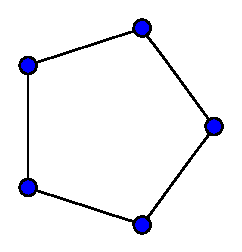
\includegraphics[width=0.25\textwidth]{pentagon.eps}
  \caption{The Pentagon}
  \label{fig:pentagon}
\end{figure}

\begin{remark}[Notation]
  Let $G$ be a graph.

  % reword access, ensure that these accessors are useful
  \begin{itemize}
  \item Let $G = (V,E)$ be a graph. For convenience, we will use subscript
    notation to refer to the edge and vertex sets of $G$, i.e. $V_G = V$ and
    $E_G = E$.
  \item $v \in G$ is an equivalent statement to $v \in V_G$
  \item $|G|$, called the \textbf{order} of $G$, is equal to $|V_G|$.
  \end{itemize}
\end{remark}

When we speak about graphs, we are concerned with the structure of the graph
rather than the specific symbols in its vertex set. Thus we use the following
definition of equality.

\begin{definition}[Equivalence of graphs]
  Two graphs $G_1$ and $G_2$ are equivalent if there exists a bijection $\phi : G_1 \to G_2$
  such that $(u,v) \in G_1$ if and only if $(\phi(u),\phi(v)) \in G_2$.
\end{definition}

Equivalence of graphs induces an equivalence relation on the set of all graphs. For convenience, we
will often only discuss graphs up to this equivalence relation (which only affects vertex labels).

\begin{example}
  The \textbf{empty graph} of order $n$ is the graph such that $|V| = n$ and $E
  = \varnothing$.

  The \textbf{complete graph} or order $n$, denoted $K_n$, is the graph containing every possible
  edge, so that $|E_{K_n}| = \frac{n(n-1)}{2}$.

  We say a graph is \textbf{bipartite} when there exists a bipartition of its vertex set such that
  there are no edges between vertices in the same part. The \textbf{complete bipartite graph},
  denoted $K_{n,m}$, is such a graph where the two partitions have cardinality $n$ and $m$
  respectively, and every pair of vertices in distinct partitions is joined by an edge.
\end{example}

\begin{figure}[H]
  \centering
  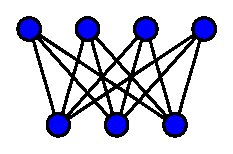
\includegraphics[width=0.4\textwidth]{k34.eps}
  \caption{The complete bipartite graph $K_{3,4}$}
  \label{fig:k34}
\end{figure}

\begin{definition}
  The \textbf{neighborhood} of a vertex $u \in G$, denoted $N(u)$, is the set of all vertices $v$
  such that $\{u,v\} \in E_G$, and these $v$ are called the neighbors of $u$. The \textbf{degree} of
  $u$ is defined by $\deg(u) = |N(u)|$. A graph in which every vertex has the same degree is
  \textbf{regular}. If that degree is equal to $k$, then the graph is said to be $k$-\textbf{regular}.
\end{definition}

\begin{example}
  $K_n$ is an $(n-1)$-regular graph, $K_{n,n}$ is an $n$-regular graph, and the pentagon is a
  $2$-regular graph.
\end{example}

\begin{definition}
  A \textbf{walk} of a graph $G$ is an alternating sequence of edges and vertices such that each
  vertex is incident to the edges before and after it.

  A \textbf{path} is the sequence of edges in a walk where every vertex is unique.

  The \textbf{shortest-path distance} between two vertices $u,v \in G$, denoted $\spd(u,v)$, is the
  minimum number of edges in a path from $u$ to $v$.
\end{definition}

\begin{definition}
  The \textbf{adjacency matrix} $A$ of a graph $G$ is given by
  \[
    A_{ij} = \begin{cases}
      1 &: \{v_i,v_j\} ~\text{is an edge in $G$} \\
      0 &: \text{otherwise} \\
    \end{cases}
  \]

  where the set $\{v_i\}_{i=1}^{|G|}$ is an ordering of the vertices in $G$.
\end{definition}
 
%% Adjacency matrix properties
% - symmetric, (eigenvalues are real)
% - eigenvectors
% - spectral gap (+ defn)
% - example: k-regular graphs have largest (simple?) eigenvalue

Note that the adjacency matrix of a graph is not unique in general. Depending on
the way that the vertices of $G$ are numbered, we may end up with a different
matrix. However, for every adjacency matrix the following holds:


\begin{definition}
  A matrix is \textbf{reducible} if and only if it can be put in block upper triangular
  form by simultaneous row and column permutations. In other words, a matrix $M$
  is reducible if and only if there exists a permutation matrix $P$ such that
  $P^{-1}MP$ is block upper triangular. Otherwise, it is said to be
  \textbf{irreducible}.
\end{definition}

\begin{proposition}
  Let $A$ be the adjacency matrix of a graph $G$. Then the following is true:

  \begin{enumerate}
  \item $A$ is symmetric (so the eigenvalues of $A$ are real)
  \item $A$ corresponds to a graph that is unique up to equivalence
  \item $A$ is irreducible if and only if $G$ is connected
  \end{enumerate}
\end{proposition}

\begin{proof}
  We omit proofs for (1) and (2) as they are self-evident.

  For (3), we first observe that $P^{-1}AP$ is an adjacency matrix of a graph
  equivalent to $G$ for any permutation matrix $P$. So without loss of generality, suppose that $G$ is
  connected and $A$ is already in block upper triangular form. Then because $A$
  is symmetric, we have

  \[
    A = \begin{bmatrix}
      B & \mathbf{0} \\
      \mathbf{0} & C
    \end{bmatrix}
  \]

  where $B$, $C$, are square block matrices. Say that $B$ has size $m \times m$. It is clear that
  there are no edges connecting the vertices in $\{1, ..., m\}$ to those in $\{m+1, ..., n\}$. Thus
  $G$ is not connected, which is a contradiction.
\end{proof}

The irreducibility result allows us to apply the Perron-Frobenius Theorem, resulting immediately in
these additional properties of $A$.

\begin{theorem}[Pg 673 (section 8.3) of ~\cite{alma991790573504746}]
  Let $A$ be an irreducible nonnegative square matrix of order $n$. The
  following is true.

  \begin{enumerate}
  \item Let $r$ be the maximum magnitude of the eigenvalues of $A$. Then $r$ is
    a (real, positive) simple eigenvalue of $A$.
  \item The eigenvalue $r$ has left and right eigenvectors whose components are
    all positive
  \item The only eigenvectors of $A$ whose components are all positive have
    eigenvalue $r$.
  \item
    \[ \min_i \sum_j a_{ij} \leq r \leq \max_i \sum_j a_{ij} \].
  \end{enumerate}
\end{theorem}

Because $A$ is nonnegative and irreducible for all connected graphs, these
properties hold for all such adjacency matrices. Indeed, the irreducibility and
nonnegativity of $A$ yields many other interesting properties which we omit
here.

\begin{definition}
  The \textbf{spectral gap} of a matrix $A$ is $\max_{i,j}|\lambda_i - \lambda_j|$, where
  $\lambda_i$ and $\lambda_j$ are the two largest eigenvalues of $G$.

  The \textbf{spectral gap of a graph} is the spectral gap of its adjacency matrix.
\end{definition}

We will next explore graph Laplacians, whose spectra are closely related to
those of adjacency matrices.

\begin{definition}
  The \textbf{degree matrix} of $G$ is the diagonal matrix defined by
  \[
    D_{ij} = \begin{cases}
      \deg(i) &: i = j \\
      0 &: i \neq j
    \end{cases}
  \]
\end{definition}

\begin{definition}
  The \textbf{graph laplacian} of $G$ is given by $L = D - A$, where $D$ is the
  degree matrix of $G$ and $A$ is the adjacency matrix. In other words,

  \[
    L_{ij} = \begin{cases}
      \deg(i) &: i=j \\
      -1 &: (i,j) ~\text{is an edge in $G$} \\
      0 &: \text{otherwise}
    \end{cases}
  \]
\end{definition}

\begin{proposition}
  %%%%% \begin{enumerate}
  %%%%%   \item 
  %%%%% \end{enumerate}
  Let $G$ be a $k$-regular graph, $\{\lambda_i\}$ and $\{x_i\}$ be the sets of eigenvalues and
  eigenvectors for its adjacency matrix $A$, and $L$ be the graph Laplacian of $G$. Then
  \begin{enumerate}
  \item $\{\lambda_i - k\}$ is the eigenvalue set of $L$, and
  \item $\{x_i\}$ is the eigenvector set of $L$
  \item $L$ and $A$ have the same spectral gap
  \end{enumerate}
\end{proposition}

\begin{proof}
  Because $G$ is regular, the degree matrix $D$ is equal to $kI$. Let ant $x_i$ be given. Then
  \begin{align*}
    Lx_i &= (A-D)x_i \\
         &= \lambda_ix_i - kx_i \\
         &= (\lambda_i - k)x_i
  \end{align*}

  Which simultaneously shows (1) and (2). (3) follows trivially from (1).
\end{proof}

%% Graph laplacian discussion
% adjacency and eigenvalues relationship

% relationship between graph laplacian eigenvalues & spectracl gap

% eigenvalue distribution of A or L

% Wigner distribution for graph eigenvalues

% see random matrix theory "semicircle law"

% what happens when this is exponential?


\section{Small-World and Scale-free Networks}
\label{sec:small_world}

Small-world networks are a class of graphs characterized by having a very small
average shortest-path distance between any two vertices compared to the overall
size of the graph.

% eigenvalues and eigenvectors

\begin{definition}
  The \textbf{characteristic path length} of a graph $G = (V,E)$ is the average
  distance between vertices in the graph, which is given by

  \[ L_G = \frac{1}{|E|} \sum_{\substack{u,v \in V \\ u \neq v}} \dist(u,v)\]

  where $\dist(u,v)$ is shortest-path distance. 
\end{definition}

\begin{definition}[Page 1 of ~\cite{PhysRevLett.90.058701}]
  Consider a graph $G = (V,E)$. $G$ is a \textbf{small-world network} if
  $L_G \sim \log{|V|}$.
\end{definition}

Small-world networks are ubiquitous in a variety of applications areas. However, many real-world
examples of such graphs also have other distinctive structural properties which are not necessarily
captured by their small-worldedness alone ~\cite{Barabasi509}. Thus, we introduce the following
definition:


% We can partially describe this structure in terms of the
% clustering coefficient.

% \begin{definition}
%   Let $v$ be a vertex in a graph $G = (V,E)$.

%   Consider the subgraph formed by the neighborhood of $v$. This subgraph has at
%   most $\deg(v)(\deg(v) - 1)$ edges, which happens when it is a clique. Denote
%   the number of edges of the neighborhood subgraph by $E_{N(v)}$.

%   The \textbf{clustering coefficient} $C_v$ is defined by
%   $C_v = \frac{E_{N(v)}}{\deg(v)(\deg(v) - 1)}$, that is, $C_v$ is the
%   proportion of edges in the neighborhood subgraph out of all possible edges.
%   The clustering coefficient of $G$ is the average of all vertex clustering
%   coefficients, $C_G = \frac{\sum_{v \in V}{C_v}}{|V|}$.
% \end{definition}

\begin{definition}[Pg. 1 of ~\cite{PhysRevE.71.027103}]
  A \textbf{scale-free network} is a graph whose vertex degrees follow a power
  law. That is, given a randomly selected $u \in G$,
  $P(\deg(u) = k) \sim k^{-\gamma}$ for some $\gamma > 0$.
\end{definition}

One of the defining characteristics of power law distributions is that they have
very long tails. In a scale-free graph with many vertices, this implies the
existence of \textbf{hubs}, which we informally define as vertices whose degrees
are far larger than average in the graph.

Real world examples of scale-free networks are abundant and include the world
wide web, cellular communication networks, and protein-protein interaction (PPI)
networks. It is not surprising, then, that scale-free networks are necessarily
small-world networks, however we defer to Cohen and Havlin for proof of this
fact.

\begin{theorem}[Final result of ~\cite{PhysRevLett.90.058701}]
  Scale-free networks are small-world networks.
\end{theorem}



\section{Random Graphs}
\label{sec:random_graphs}

% exponential distribution eigenvalues

\begin{definition}
  A \textbf{random graph} is a random variable for which all outcomes are
  undirected graphs.

  A \textbf{random graph process}, denoted $(G_t)$, is a family of random graphs
  indexed by a discrete time $t \in \mathbb{N}$.
\end{definition}

We are interested in random graph processes which build small-world networks.
The Watts-Strogatz graphs are an example of such a process. They are defined by
starting with a regular ring lattice and randomly rewiring edges until the graph
is obtained.

\begin{definition}
  An $n$-$k$ \textbf{regular ring lattice} is a graph $(V, E)$ with $n$ vertices
  such that $u,v$ is an edge if and only if $|u-v| \leq \frac{k}{2}$.
\end{definition}

\begin{definition}
  Let $v$ be a vertex in a graph. We can \textbf{rewire} $v$ by deleting one
  edge of $v$ and drawing a new one by sampling uniformly from all vertices that
  do not share an edge with $v$.
\end{definition}

\begin{definition}
  Given a probability $p$ and regular ring lattice parameters $n$ and $k$, we
  define the $(n,k,p)$ \textbf{Watts-Strogatz Process} as follows.

  Let $r(G,v)$ be a random process that rewires vertex $v$ in a graph $G$. We
  define a family of graphs, $(G_t)$, by

  \[
    G_{t+1} = \left\{
      \begin{array}{lc}
        r(G_t,t) &: X \leq p \\
        G_t &: X > p
      \end{array}
    \right.
  \]

  for $t = 1,\dots, |G|$, where $G_0$ is the $n$-$k$ regular ring lattice, and
  $X$ is a uniform random variable in the range $[0,1]$. That is, we iterate
  over the vertices of the ring lattice and rewire each one with probability
  $p$.

  We call graphs sampled from $G_{|n|}$ \textbf{Watts-Strogatz graphs}.
\end{definition}

Watts and Strogatz showed empirically that the Watts-Strogatz graphs are small-world networks for all
but extremely small values of $p$~\cite{Watts1998Collective}. However, in general, they are not scale
free networks~\cite{Barabasi509}, and thus do not show the structural characteristics of many
practical data sets.

% TODO: ask about restated definitions
\begin{definition}[Pg. 511 of ~\cite{Barabasi509}]
  \label{def:ba}
  Let any graph $G_0$ be given as well as some parameter $m$, $m \leq |G_0|$. We
  build the random graph $G_{t+1}$ by adding a new vertex to $G_t$ and
  connecting it to $m$ vertices of $G_t$ with probabilities proportional to the
  degree of each vertex. That is, the probability of adding an edge to a vertex
  $u$ is

  \[
    p_u = \frac{\deg(v)}{\sum_{v \in G_t} \deg(v)}
  \]

  on the first step, and this is done a total of m times without replacement.

  We call $(G_t)$ the $(G_o,m)$-\textbf{Barab\'asi-Albert (BA) process} and graphs
  sampled from $G_n$ $(G_o,m,n)$-\textbf{Barab\'asi-Albert (BA) graphs}.
\end{definition}

This type of model, where edges to a new vertex are drawn with non-uniform
probability, is known as \textbf{preferential attachment}.

\begin{theorem}[Pg. 511 of ~\cite{Barabasi509}]
  \textbf{Barab\'asi-Albert graphs} are scale-free
\end{theorem}

The scale-free-ness of BA graphs makes them an attractive model, as they are likely to have degree
distributions similar to those of many real data sets. In addition, BA graphs are guaranteed to be
connected.

%%% Local Variables:
%%% mode: latex
%%% TeX-master: "../Main"
%%% End:



\chapter{Random Labeled Graphs}

% introduction to random graphs and our models
We wish to use random graphs to test vertex classifiers. An issue that arises is that the generative
models presented so far do not suggest any natural labeling for the vertices of the resultant graphs.
Thus, we propose some models for generating labeled small-world and scale-free networks.

\begin{definition}
  A \textbf{labeled graph} is a graph $G$ and a function $c : V_G \to S$, where $S$ is an arbitrary.
  For $u \in V_G$, we call $c(u)$ the \textbf{class} of $u$.
\end{definition}

In considering labeled graphs, it is useful to look at not only at each vertex's degree, but also the
number of neighbors with the same label vs the number of neighbors with a different label. For
convenience, we define these quantities as follows:

\begin{definition}
  Let $G$ be a labeled graph, $u \in V_G$. The \textbf{same-class degree} of $u$, $\deg_{same}(u)$, is
  the number of vertices in the neighborhood of $u$ in the same class as $u$. $\deg_{diff}(u) =
  \deg(u) - \deg_{same}(u)$ is the number of vertices in a different class.
\end{definition}


\begin{definition}
  Let $m$ be a natural number. We construct the \textbf{complete components
    graph} of order $n = 2m$ as follows. Let $V = \{1,2, ..., 2m\}$, and then define
  $E$ by

  \[
    E = \{ (u,v) : u,v \in \{1,...,m\} ~\text{or}~ u,v \in \{m+1,...,2m\} \}
  \]

  i.e. the disjoint union of two complete graphs of order $m$. In addition, we label the graph by the
  function

  \[c(u) = \left\{
      \begin{cases}
        0 &: u \in \{1,...,m\} \\
        1 &: u \in \{m+1,...,2m\}
      \end{cases}
    \right.\]
\end{definition}

\begin{definition}
  \label{def:ncc}
  Let parameters $(m,p,q)$ be given, $m \in \mathbb{N}$ and $p,q \in [0,1]$, and let $G_0$ be the
  complete components graph of order $2m$. We construct a \textbf{Noisy Complete Components (NCC)}
  graphs as follows.

  Iterate over ever pair of vertices in the graph (i.e. the edge set of
  $K_{2m}$). For every pair $(u,v) \in E_{G_0}$, that is, for the edges that
  already exist in $G_0$, we delete the edge with probability $q$. Likewise, for
  each pair $(u,v) \notin E_{G_0}$, we add the edge $(u,v)$ with probability
  $p$.

  The resultant graph is an NCC graph.
\end{definition}

We will now inspect the properties of such graphs in order to demonstrate that they are, in fact,
small worlds graphs in the subset of the parameter space in which we're interested.

\textbf{Question for Profs. Walls \& \'O Cath\'ain} Should I define the binomial and Bernoulli
distributions? If so, how much detail? Are the PMFs sufficient?

\begin{theorem}
  \label{thm:ncc_deg}
  Let $G$ be an $(m,p,q)$ NCC graph and $u$ a vertex in $G$. Then $\deg(u)$ follows the distribution
  $X + Y$, where $X$ and $Y$ are (independent) binomial random variables, $X \sim B(m-1,1-q)$ and
  $Y \sim B(m,p)$. Moreover, $\deg_{same}(u) = X$ and $\deg_{diff}(u) = Y$.
\end{theorem}
\begin{proof}
  First, observe that adding and deleting edges to an NCC graph is done independently for each edge.
  In other words, the existence or nonexistence of any edge of $G$ is independent of every other edge.
  In addition, the number of edges added between $u$ and all other different-class vertices is equal
  to a sum of $m$ Bernoulli random variables of probability $p$, because there are $m$ possible edges
  from $u$ to the opposite class. Thus $deg_{diff}(u)$ follows a binomial distribution on $m$ trials,
  $deg_{diff}(u) = Y \sim B(m,p)$.

  In the case of same-class edges, we will consider the probability that an edge is \textit{preserved}
  rather than deleted. Edges are preserved with probability $(1-q)$, so as in the different-class
  case, we can see that the same-class degree of $u$ follows a binomial distribution on $(m-1)$
  trials, $deg_{same} = X \sim B(m-1,1-q)$.

  As we've counted both the same- and different-class degrees, it is clear that $deg(u) = X + Y$.
\end{proof}

We must take care to note that this is not the same thing as the degree distribution over the whole
graph $G$. While each edge with respect to a single vertex is picked independently, this is not true
over the whole graph, since each edge is connected to two vertices.

\begin{remark}
  The previous theorem shows that the following is true
  \begin{enumerate}
  \item $\E(\deg_{same}(u)) = (m-1)(1-q)$ and $\E(\deg_{diff}(u)) = mp$, where $\E$ is expectation.
  \item $\Var(\deg_{same}(u)) = (m-1)(1-q)q$ and $\Var(\deg_{diff}(u)) = mp(1-p)$, where $\Var$ is
    variance.
  \item $\E(\deg(u)) = (m-1)(1-q) + mp$ by linearity of expectation.
  \item $\Var(\deg(u)) = (m-1)(1-q)q + mp(1-p)$ by linearity of variance on independent random
    variables.
  \end{enumerate}
\end{remark}

\begin{theorem}
  Let $u$ and $v$ be vertices in an $(m,p,q)$ NCC graph. We write $P(\spd(u,v) = k)$ for the probability
  that the shortest path between $u$ and $v$ is equal to $k$.

  If $c(u) = c(v)$, then $\E(P(\spd(u,v) = 1)) = 1-q$ and
  $\E(P(\spd(u,v) = 2)) = 1- (1 - (1-q)^2)^{m-1} (1-p^2)^{m}$.

  If $c(u) \neq c(v)$, then $\E(P(\spd(u,v) = 1)) = mp$ and
  $\E(P(\spd(u,v) = 2)) = 1- ((1-q)(1-p) + q)^{m-1}(pq+(1-p))^n$.
\end{theorem}
\begin{proof}
  For the cases where $\spd(u,v) = 1$, the results follow immediately from definition \ref{def:ncc}.

  \textbf{Note to Professors:} while typing this, I found an error. I need to nudge around the random
  variables in the probability formulas because I'm operating under the assumption that 1) there's an
  edge between $u$ and each neighbor, and 2) there's not an edge between $u$ and $v$. This just
  reduces the number of trials on the binomial variables so it should just be changes by factors of $p$
  and $q$, but I didn't have time to work it out.

  % TODO: fix this. X changes slightly because we assume that the trial between u and v failed, and
  % the trial between u and each neighbor succeeded.
  Now, we consider the case where $\spd(u,v) = 2$ and $c(u) = c(v)$. Under these circumstances, we
  denote the number of same-class neighbors by the random variable $X$ and the number of
  different-class neighbors by $Y$. A length-2 path between $u$ and $v$ must exist unless we fail to
  preserve/add every single edge from the neighborhood of $u$ to $v$, which happens with probability
  $q^X(1-p)^Y$. Thus $P(\spd(u,v) = 2) = 1 - q^X(1-p)^Y$.

  Since $X$ and $Y$ are binomial random variables by theorem \ref{thm:ncc_deg}, their probability mass
  functions are:

  \begin{align*}
    f_X(x) &= {n-1 \choose x} (1-q)^xq^{n-1-x} \\
    f_Y(y) &= {n \choose y} p^y(1-p)^{n-y}
  \end{align*}

  using the expectation formula, we can compute $q^x$ and $p^Y$:

  \begin{align*}
    \E(q^X) &= \sum_{i=0}^{n-1}q^i{n-1 \choose i}(1-q)^iq^{n-1-i} \\
            &= q^{n-1}\sum_{i=0}^{n-1}{n-1 \choose i}(1-q)^i(1)^{n-1-i} \\
            &= q^{n-1}(2-q)^{n-1} \\
            &= (1 - (1 - q)^2)^{n-1}
  \end{align*}

  \begin{align*}
    \E((1-p)^Y) &= \sum_{i=0}^{n}(1-p)^i{n \choose i}(1-(1-p))^i(1-p)^{n-i} \\
            &= (1-p)^{n}\sum_{i=0}^{n}{n \choose i}(1-(1-p))^i(1)^{n-i} \\
            &= (1-p)^{n}(p-1))^{n} \\
            &= (1 - p^2)^{n}
  \end{align*}
  thus, in this case,

  \[ P(\spd(u,v) = 2) = 1 - (1 - (1-q)^2)^{n-1}(1-p^2)^n \]

  % TODO: fix this. Y changes slightly because we assume that the trial between u and v failed.
  In the case where $c(u) \neq c(v)$, the probability becomes $P(\spd(u,v) = 2) = 1 - q^Y(1-p)^X$, so
  by an analogous computation, we get

  \[ P(\spd(u,v) = 2) = 1 - (q + (1-p)(1-q))^{n-1}(pq + (1-p))^n \]
\end{proof}


However, these graphs are extremely regular, so they do not exhibit scale-free properties. Thus, we
also propose a variant on the Barab\'asi-Albert model which adds labels while preserving the power law
degree distribution.

%% prove theorem: the following are equal: frobenius norm of a matrix,
%% \sum{\lambda^2}, number of edges in G (or something like this)

% sketch: recall \sum \lambda_i = \tr(M). Consider A^2, whose trace is the sum
% of degrees

% TODO: refer back to previous chapter definition of BA 
\begin{definition}
  Let parameters $G_0$ and $m \leq |G_0|$ be given as in the BA process as well
  as a finite set of labels $S$ and a factor $\rho \ge 1$. In addition, suppose
  each vertex in $G_0$ has been labeled by an element of $S$. Given a graph
  $G_t$, we build $G_{t+1}$ as follows.

  As in the BA process (see definition \ref{def:ba}, page \pageref{def:ba}), we will add one new vertex and draw
  edges using preferential attachment, however, we label our new vertex $l$, which is chosen from $S$
  with uniform probability. Then, we reweight the probability of drawing each edge in order to favor
  vertices with label $l$ by a factor of $\rho$.

  Define $S_l$ to be the set of vertices with label $l$. Then, we define the
  probability of drawing an edge to a vertex $u$ as

  \[
    p_u = \begin{cases}
      \frac{\rho\deg(u)}{w} &: u \in S_l\\
      
      \frac{\deg(u)}{w} &: u \in (V_G - S_l)\\
    \end{cases}
  \]

  where $w$ is the weighted degree sum,

  \[
    w = \rho \sum_{v \in S_l}\deg(v) + \sum_{v \in (V_G - S_l)}\deg(v)
  \]

  We call this random process the \textbf{class-weighted Barab\'asi-Albert
    (CWBA) process} and we call graphs sampled from this model \textbf{CWBA
    graphs}.

  % TODO: add example
\end{definition}

%%% Local Variables:
%%% mode: latex
%%% TeX-master: "../Main"
%%% End:

% do DSD in terms of eigenvalues and spectral gap (regular case first)
%  keep the circulant graphs
\chapter{Metrics on Graphs}

\section{Definition of DSD}
\subsection*{Definition of DSD}

\noindent In their original definition, Cao et al. define DSD in terms of a
vector-valued function $\mathrm{He}^{k}(u)$, which computes the expected number of times
a length-$k$ random walk originating at a vertex $u$ will visit each other vertex
in the graph. They compute DSD by taking the $l_1$-norm of the difference
between two such vectors in the limit as $k \to \infty$. We present an
alternative definition which is more compact and easier to manipulate with the
usual machinery of linear algebra.

Random walks can be modeled as Markov chains, where the current state is a
vertex $u$ in the graph, and the transition probability is $\frac{1}{\deg(u)}$
for the neighbors of $u$ and $0$ otherwise. The transition matrix can be written
$T = AD$, where $A$ is the adjacency matrix of the graph and $D$ is the unique
diagonal matrix such that every column of $T$ sums to 1 (i.e.
$D_{u,u}=\frac{1}{deg(u)}$, or equivalently, $D$ is the inverse of the degree
matrix). For our purposes, we assume that vertices are labeled by the positive
integers $1,2,...,n$ and that the rows and columns of the $G$ correspond to this
ordering.

The marginal distribution of vertices in the $k\nth$ step of a random walk
originating from vertex $u$ is given by $T^ke_u$, where $e_u$ is the initial
state vector, which is the $u\nth$ standard basis vector in $\R^n$,
$e_{u,u} := 1$ and $e_{u,j} := 0, u \neq j$ for $u=1,...,n$.

Thus, we can define the DSD, $\delta(u,v)$, by

\[
  \delta(u,v) = ||\sum_{k =0}^{\infty}{T^ke_u - T^ke_v}||_1
\]

\subsection{Proof that DSD is a Metric}

A metric is a nonnegative real-valued function that generalizes Euclidean
distance between points in $R^n$ to general sets. In our case, the set is the
vertices of the graph. Metrics allow us to define metric spaces which are
generally useful, but the context of our problem, we are mainly interested in
them because they allow us to partially order all vertices in a graph based on
their distance from a fixed vertex.

\begin{definition}
  A \textbf{metric} with respect to a set $S$ is a function $d : S x S \to \R$
  satisfying

  \begin{enumerate}
  \item $d(u,v)\geq 0 ~ \forall u,v \in G$,
  \item $d(u,v) = 0 \iff u = v$ (identity of indiscernables),
  \item $d(u,v) = \delta(v,u) ~\forall u,v \in G$, and
  \item $d(u,v) \leq \delta(u,w) + \delta(v,w) ~\forall u,v,w \in G$
    (triangle inequality).
  \end{enumerate}\end{definition}

First, we will define a finite analog to the $\mathrm{He(u)}$ vectors of Cao et al. Because
$T$ is a transition matrix for a Markov chain, this means that
$\lim_{k \to \infty} T^k$ converges to a stationary distribution which we will
call $T^\infty$.

\begin{lemma}
  Let $T$ be a transition matrix for a markov chain and $T^\infty$ the
  corresponding stationary distribution. The matrix sum

  \[
    S = \sum_{k=0}^{\infty}(T^k - T^\infty)
  \]

  converges.
\end{lemma}
\begin{proof}
  \textbf{TODO} [I thought this was an easy proof, but now I'm not sure -- JP]
\end{proof}

\begin{remark}
  $S$ is symmetric.
\end{remark}
\begin{proof}
  Clearly, since $T$ is symmetric and commutes with itself, $T^k$ is symmetric
  for all $k$. This implies that $T^\infty$ is also symmetric, as is the
  difference $T^k - T^\infty$ for all $k$. Thus, every term in the sum is
  symmetric, completing the proof.
\end{proof}

We will denote row vectors of matrices with a single subscript, i.e. $S_u$ is
the $u\nth$ row of $S$ which is equal to the $u\nth$ column. The columns of $S$
are our finite analog for the $\mathrm{He}$ vectors. Now, note that $T^ke_u$ is
equal to $T^k_u$. This allows us to rewrite DSD as

\begin{align*}
  \delta(u,v) &= ||\sum_{k=0}^{\infty}((T^k)_u - (T^k)_v)||_1 \\
              &= ||\sum_{k=0}^{\infty}((T^k-T^\infty)_u - (T^k-T^\infty)_v)||_1 \\
              &= ||S_u - S_v||_1
\end{align*}

\begin{theorem}
  DSD is a metric.
\end{theorem}
\begin{proof}
  We must show:

  \begin{enumerate}
  \item $\delta(u,v)\geq 0 ~ \forall u,v \in G$,
  \item $\delta(u,v) = 0 \iff u = v$ (identity of indiscernables),
  \item $\delta(u,v) = \delta(v,u) ~\forall u,v \in G$, and
  \item $\delta(u,v) \leq \delta(u,w) + \delta(v,w) ~\forall u,v,w \in G$
    (triangle inequality).
  \end{enumerate}

  Let $G = (V,E)$ be an arbitrary graph of order $n$ and define $T$, $T^\infty$,
  and $S$ as above. We define a map $f : V \to \R^n$ by $f(u) = S_u$. DSD is
  equivalent to taking the $l_1$-norm of differences between these points. Since
  $l_1$ distance is a metric in $\R^n$, we have shown (1), (3), and (4).

  Because $T$ is invertible, no two rows or columns of $T$ are equal, which also
  applies to the powers of $T$. Consequently, $S$ is also invertible. Thus,
  $f$ is injective, proving (2).

  % The eigenvectors of $T$ span $\R^n$, which also means that no two
  % rows of $T$ are equal, as otherwise $\dim T$ would be less than $n$. We
  % rewrite every row/column $T_u$ as a linear combination
  % \[
  %   T_u = \sum_{i=1}^n \theta_i(u) x_i
  % \]

  % for some coefficient vector $\theta(u)$, where $x_i$ are eigenvectors of $T$.
  % Let $\lambda_i$ be the respective eigenvalues. Because all the rows in $T$ are
  % distinct, every coefficient vector $\theta(u)$ is distinct. Also, the
  % corresponding coefficients for powers of $T$ are
  % $T^k_u = \sum{\lambda_i^{k-1} \theta_i(u) x_i}$.

  % Let $k$ be arbitrary, and suppose $T^k_u = T^k_v$ for some $u \neq v$. Then
  % $\lambda_i^{k-1}\theta_i(u) = \lambda_i^{k-1}\theta_i(v)$ for all
  % $i = 1,...,n$. Clearly, this only holds for the case that
  % $\theta_i(u) = \theta_i(v)$ for all $i$, which is a contradiction because it
  % implies $T_v = T_u$. Thus, every row (and column) of $T^k$ is distinct for all
  % powers $k$, and this property extends to $S$, thus proving (2).

\end{proof}

%%% Local Variables:
%%% mode: latex
%%% TeX-master: "../Main"
%%% End:


\section{DSD on Special Graphs}
\subsection{Complete Graphs}
Consider the complete graph $K_n$. In this case, $D = \frac{1}{n-1}I$ and
$A = (J - I)$, so $T=\frac{1}{n-1}(J-I)$. In order to compute $T^ke_u$ in the
limit, we will represent $e_u$ as a linear combination of eigenvectors of $A$.

\begin{remark}
  $1_n$ is an eigenvector of $T$ with eigenvalue $\lambda = 1$, and every
  vector $x \in \R^n$ such that $\sum_i x_i = 0$ is an eigenvector of $T$ with
  $\lambda = -\frac{1}{n-1}$.
\end{remark}
\begin{proof}
  Multiplying a vector by the all-ones matrix takes the sum of that vector's
  values for every index in the result, so $J \cdot 1_n = n \cdot 1_n$.
  Similarly $Jx = 0_n$, for any $x$ s.t. $\sum_i x_i = 0$. Thus,

  \begin{align*}
    T\cdot 1_n &= \frac{1}{n-1}(J-I) \cdot 1_n \\
               &= \frac{1}{n-1}(n\cdot 1_n - 1_n) \\
               &= 1_n
  \end{align*}

  and

  \begin{align*}
    Tx &= \frac{1}{n-1}(J-I)x \\
       &= \frac{1}{n-1}(0_n - x) \\
       &= -\frac{1}{n-1}x
  \end{align*}
\end{proof}


Next, we will show how to write any $e_u$ as a linear combination of
eigenvectors of $T$. We define $\alpha_u$ by $\alpha_{u,u} := n-1$ and
$\alpha_{u,j} = -1, u\neq j$. The entries of $\alpha_u$ sum to $0$, so
$T\alpha_u=-\frac{1}{n-1}\alpha_u$. We can write
$e_u = \frac{1}{n}(1_n + \alpha_u)$.

\begin{corollary}
  The eigenvectors of $J-I$ span $\R^n$.
\end{corollary}
\begin{proof}
  Since all standard basis elements $e_j$ of $\R^n$ can be expressed as linear
  combinations of eigenvectors for $J-I$, the eigenvectors of $J-I$ span $\R^n$.
\end{proof}

\begin{theorem}
  Let $K_n$ be the complete graph with nodes labelled $1,...,n$. Then for any
  two distinct nodes $u$ and $v$, $\delta(u,v) = \frac{2(n-1)}{n}$.
\end{theorem}
\begin{proof}
  We will use $\alpha_u$ as defined above. DSD is given by

\begin{align*}
  \delta(u,v) &= \sum_{k = 0}^{\infty}{||T^ke_u - T^ke_v||_1} \\
              &= \frac{1}{n}\sum_{k = 0}^{\infty}{||T^k(1_n + \alpha_u - 1_n -
                \alpha_v)||_1}\\
              &= \frac{1}{n}\sum_{k = 0}^{\infty}{||T^k(\alpha_u - \alpha_v)||_1} \\
              &= \frac{1}{n}\sum_{k = 0}^{\infty}{||(-\frac{1}{n-1})^k(\alpha_u -
                \alpha_v)||_1} \\
              &= \frac{||\alpha_u - \alpha_v||_1}{n}
                \sum_{k = 0}^{\infty}{(-\frac{1}{n-1})^k} \\
\end{align*}

Since $|-\frac{1}{n-1}| < 1$, the geometric series converges,
$\sum_{k=0}^{\infty}(-\frac{1}{n-1})^k = \frac{n-1}{n}$. When $u \neq v$, the
difference $\alpha_u - \alpha_v$ will have exactly two non-zero entries (since
they are identical at all indices but $u$ and $v$). These non-zero entries will
be $n$ at index $u$ and $-n$ at index $v$. Thus,
$||\alpha(u)-\alpha(v)||_1 = 2n$, and so

\begin{align*}
  \delta(u,v) &= \frac{2n}{n}(\frac{n-1}{n}) \\
              &= \frac{2(n-1)}{n} \\
\end{align*}

\end{proof}

\subsection{Circulant Graphs}

Circulant graphs have well-understood spectra, so we can perform a similar
analysis to the complete case.

\begin{definition}
  We {\bf rotate} a row vector by moving each of its elements over one index to
  the right. The rightmost element wraps around and is put in the leftmost index
  in the result.
\end{definition}

\begin{example}
  The rotation of $\colvec{1 & 2 & 3 & 4}$ is $\colvec{4 & 1 & 2 & 3}$.
\end{example}

\begin{definition}
  A matrix is {\bf circulant} if each row is equal to the A graph is {\bf
    circulant} if it has a circulant adjacency matrix.
\end{definition}

\begin{example}
  The pentagon with this circulant adjacency matrix:
  \[
    \begin{bmatrix}
      0 & 1 & 0 & 0 & 1 \\
      1 & 0 & 1 & 0 & 0 \\
      0 & 1 & 0 & 1 & 0 \\
      0 & 0 & 1 & 0 & 1 \\
      1 & 0 & 0 & 1 & 0 \\
    \end{bmatrix}
  \]
\end{example}

\subsubsection*{Spectrum}

[The expressions for eigenvectors/eigenvalues are sourced from Wikipedia --JP]

All circulant matrices have the same eigenvectors given by

\[x_j = \colvec{1 \\ z^j \\ z^{2j} \\ ... \\ z^{(n-1)j}}\]

where $j=1,2,...,n$ and $z=\exp(\frac{2 \pi i}{n})$ is an $n^{th}$ root of
unity. Note that the $n^{th}$ eigenvector is $1_n$, and that multiplying $x_j$
by $z^{n-j}$ rotates it, as $1 = z^0 = z^n$. We can write our basis vectors $e_u$ as
linear combinations of elements in $x_j$ like so:

\[e_u = \frac{1}{n}(1_n + \sum^{n-1}_{j=1} z^{(u-1)(n-j)} x_j)\]

This depends on the fact that the sum of all $n^{th}$ roots of unity is 0, so
$1 + \sum_{j=1}^{n-1}z^j = 0$. Therefore, we get $ne_1$ by summing over all
eigenvectors, since every index except the first will vanish. We can get the
other basis vectors by repeatedly rotating all the eigenvectors except $1_n$,
which is where the $z^{(u-1)(n-k)}$ comes from in the form above.

The corresponding eigenvalues $\lambda_j$ depend on the matrix. Let
$r = \colvec{r_1 & r_2 & ... & r_n}$ be the first row of the matrix. Then, the
$j^{th}$ eigenvalue is given by

\[\lambda_j = \sum_{k}r_kz^{(k-1)j} \]


\subsubsection*{Cycles}

Cycles are the most obvious example of circulant graphs. The eigenvalues of a
cycle are given by $\lambda_j = z^{j-1} + z^{j+1}$.



\chapter{Label Prediction Methods on Graphs}
In this chapter, we present how we can apply the classification problem to labeled random graphs using metrics on graphs such as the Diffusion State Distance (DSD). We present our problem formulation and its relation to the topics discussed in the previous chapters.

\section{Problem Definition}
Consider an undirected connected graph $G = (V,E)$ (Chapter 2 Definition 1). A graph is \textbf{undirected} if for all edges $(u,v) \in E$, where $u,v \in V$ we have $(u,v) = (v,u)$. A graph is \textbf{connected} if there is a path (Chapter 2 Definition 4) from any $u \in V$ to any other $v \in V$, $u \neq v$. Many real world examples exist of data that can be represented as undirected graphs, and will be discussed later in this chapter. Such data may also contain information about attributes of the vertices in the graph. Yang and Leskovec~\cite{DBLP:journals/corr/abs-1205-6233} used the scientific collaboration network DBLP where authors were modeled as vertices and edges were formed between authors who had published at least one paper together. Vertices were labeled by publication venues. A construction of a graph such as this gives us a labeled graph. However, not all labels of vertices may be known. Cao, Zhang, Park, Daniels, Crovella, Cowen, and Hescott~\cite{10.1371/journal.pone.0076339} study the prediction of protein function on protein-protein interaction networks. Many protein functions, labels on the vertices of these networks, are not known. Thus, prediction algorithms are used to predict protein functions on these networks. A variety of prediction algorithms exist, but we study prediction algorithms that incorporate metrics on graphs. Lastly, prediction accuracies are computed for prediction algorithms using different metrics.


\section{Real World Data}
In this section, we discuss three different examples of graph-based studies performed on real world data. We discuss how these examples constructed graphs from their data, and what kind of studies were performed on the resulting graphs. These studies give constructions of different graph representations of data that we can use to test the effects of different metrics with prediction algorithms.

\subsection{PPI networks}
% Fix citations, one ref per page is enough
Cao, Zhang, Park, Daniels, Crovella, Cowen, and Hescott~\cite{10.1371/journal.pone.0076339} studied the prediction of protein functional labels on the \emph{S. cerevisiae} protein-protein interaction network (PPI network). The authors constructed a graph using annotated physical interactions in this PPI network. Proteins corresponded to vertices, and an annotated physical interaction between two proteins corresponded to an edge. Cao et al. removed redundant edges and the largest connected component was selected, resulting in a graph of 4990 vertices and 74,310 edges. They also noted that PPI networks are known to resemble small-world networks, as they have a small maximum shortest path, and a small characteristic path length. This implies that most vertices in the graph are close to every other vertex in the graph. Figure \ref{fig:PPI_example} shows an example of functional annotation using the DSD from Cao et al.

\begin{figure}[h]
\centering
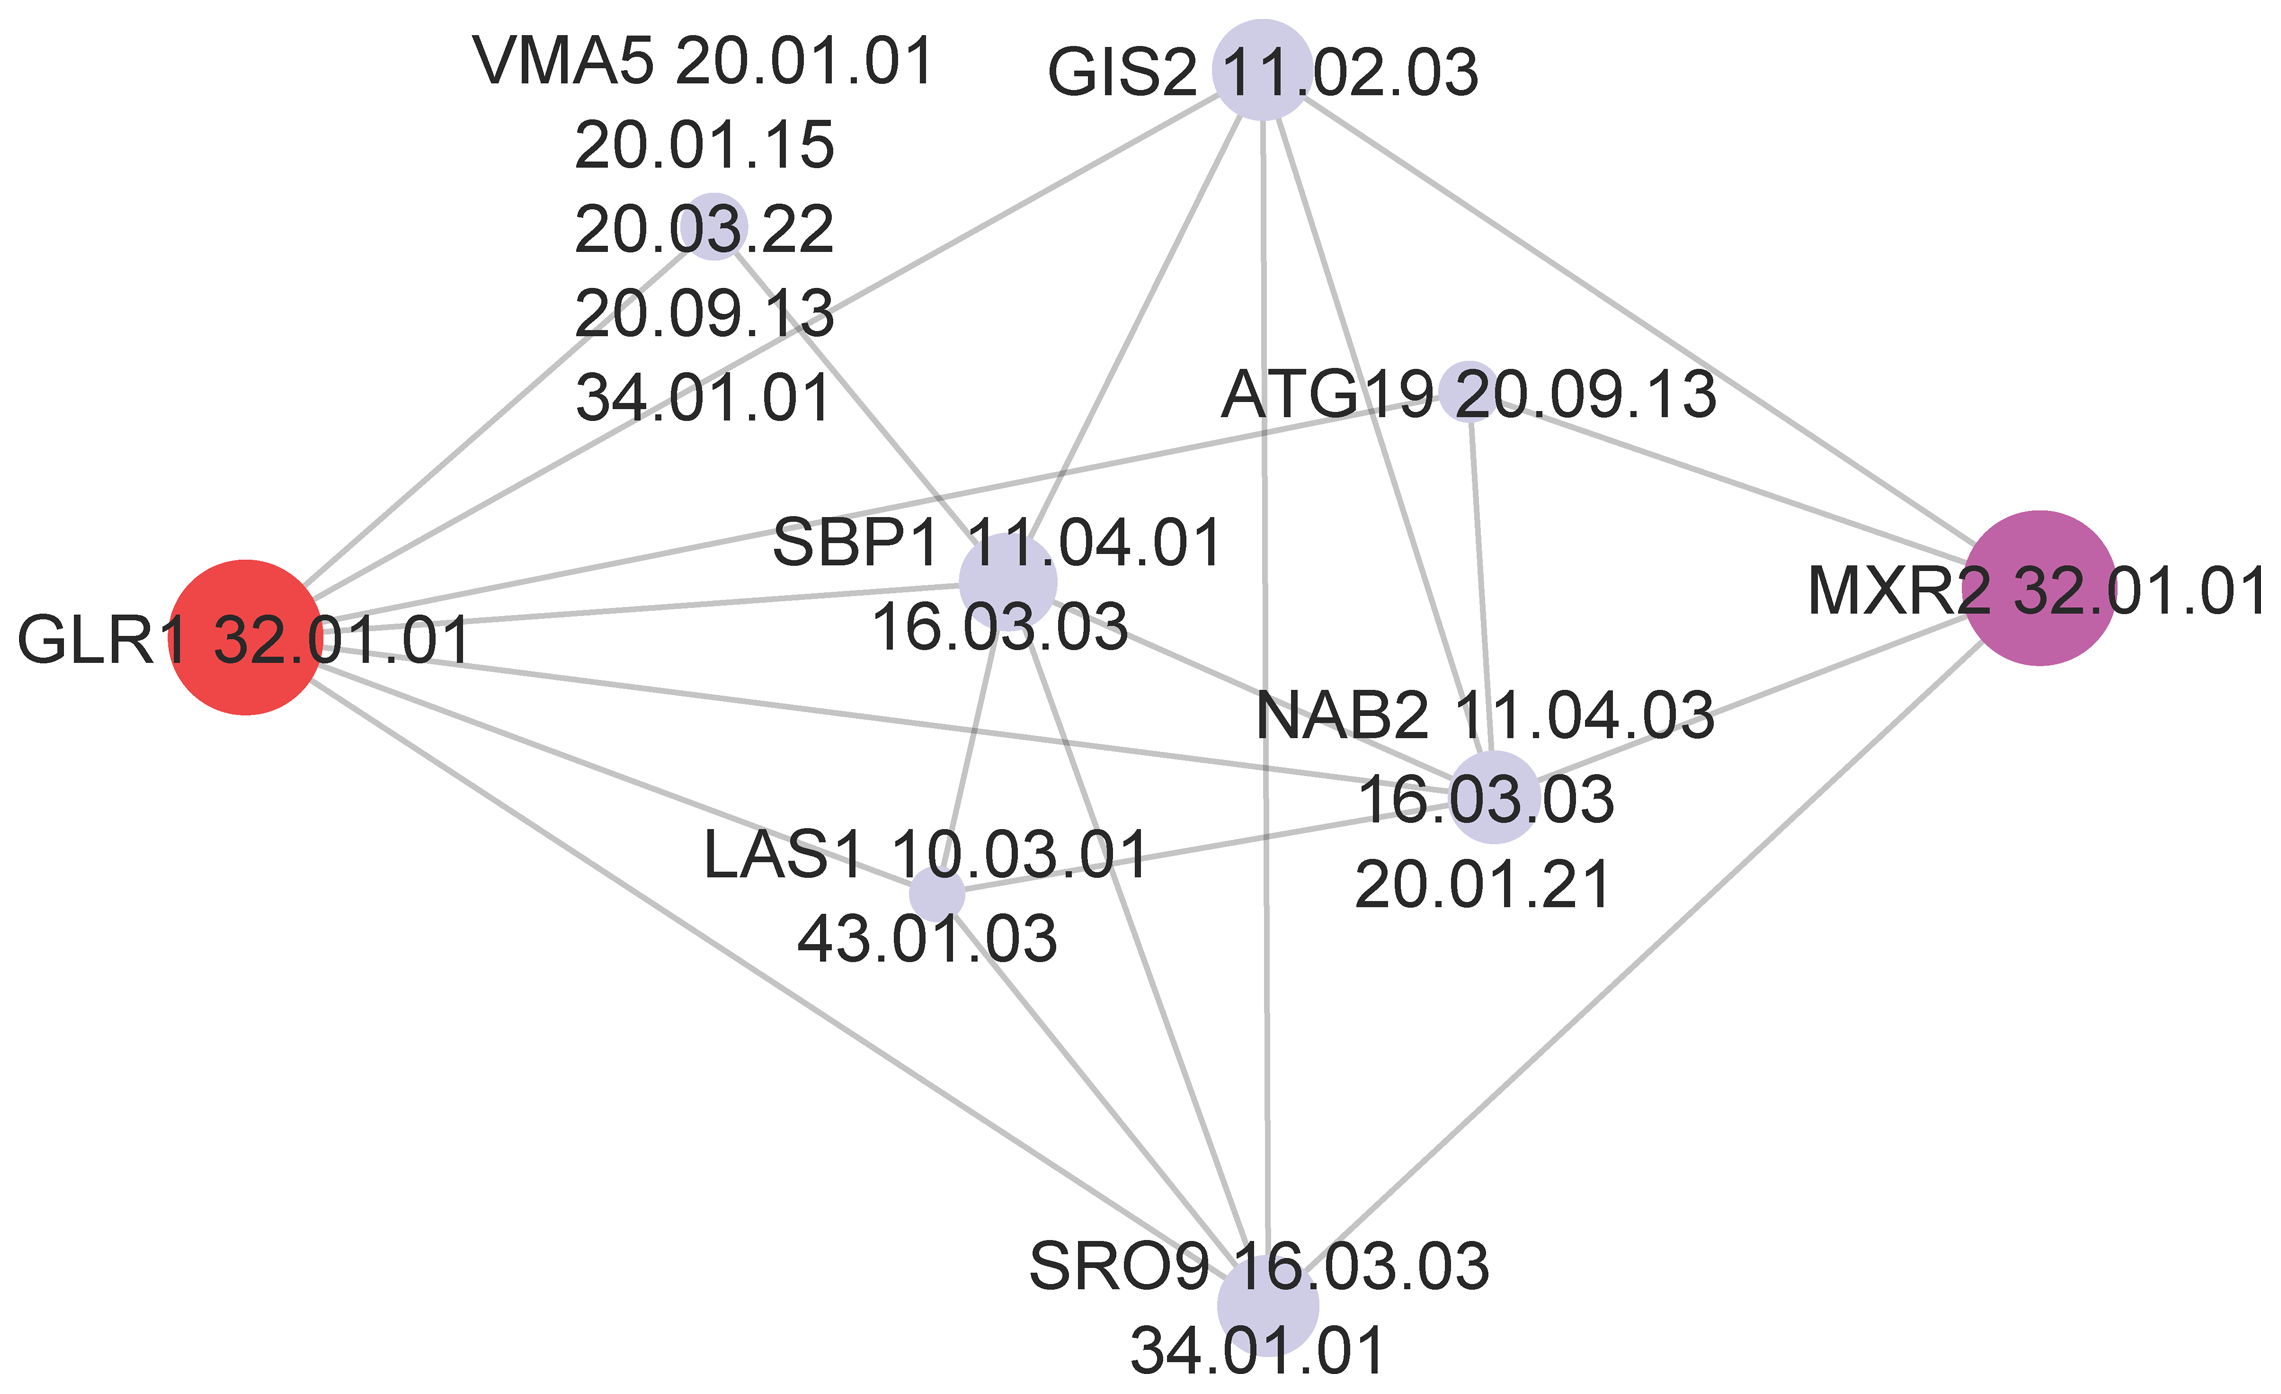
\includegraphics[width=0.75\textwidth]{dsd_ex.png}
\caption{An example of functional annotation with the DSD metric from Cao et al. ~\cite{10.1371/journal.pone.0076339}. It is clear that the vertex colored purple is not a direct neighbor of the red vertex with respect to the shortest path distance metric. However, the purple vertex has a DSD distance closest to the red vertex, and they have the same label. Meanwhile, the direct neighbors of the purple vertex have different labels.}
\label{fig:PPI_example}
\end{figure}

Cao et al. used four different prediction algorithms to compare the effectiveness of the DSD metric to that of the shortest path metric. Both weighted and unweighted majority voting algorithms, as well as the $\chi^{2}$ neighborhood algorithm, multi-way cut algorithm, and functional flow algorithm were used to compare the predictive performance of these metrics. The DSD metric was expected to perform better that the shortest path metric, since the small characteristic path length of the PPI network causes the notion of a shortest paths neighborhood to lose significance. All vertices in this network are close to every other vertex in the graph, so any neighborhood would contain a large portion of the vertices in the graph.

\subsection{Graph model for recommender systems}
Huang, Chung, and Chen~\cite{huang2004graph} introduce a generic graph model for e-commerce transaction data that can support various recommendation methods. The two-layer graph model proposed represents relationships between products and customers. In this model, each layer consists of vertices representing products or customers. Three types of edges in this two layer system capture the inputs to this model from real world data. Edges between two customers capture similarity based on available demographic data, answers to questionnaires, and web usage patterns. Edges between two products capture similarity using descriptions of the product. Finally, edges between customers and products capture transaction information such as purchase history, customer rating, and related browsing behavior. Figure \ref{fig:recommender_example} illustrates an example of the two-layer graph model.

\begin{figure}[h]
\centering
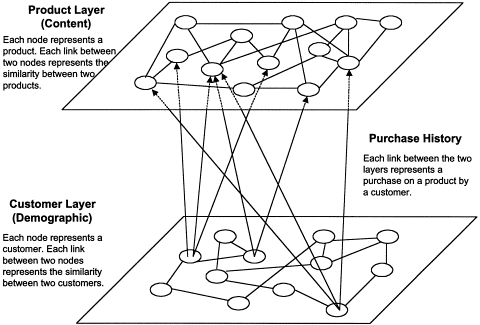
\includegraphics[width=0.75\textwidth]{recommender_ex.png}
\caption{The two-layer graph model proposed by Huang, Chung, and Chen~\cite{huang2004graph}.}
\label{fig:recommender_example}
\end{figure}

% more info
Huang, Chung, and Chen~\cite{huang2004graph} considered three different recommendation methods to use on the model mentioned previously. The direct retrieval method looks at a customer's previous purchases and products purchased by similar customers to retrieve products to recommend to the customer. The association mining method uses the purchase history of a customer to generate association rules about purchasing patterns in order to predict the customer's next purchases. The high-degree association retrieval method uses weights on edges to represent association strength and examines paths between the target customer vertex and a product vertex to calculate an association estimate and determine if the product should be recommended. Transactions from one of the largest online bookstores in Taiwan were used for data including 9695 books, 2000 customers, and 18,771 transaction records.

% Add more speculations, tie to rest of thesis
The two-layer graph model introduced by Huang, Chung, and Chen~\cite{huang2004graph} can be interpreted as a graph labeling problem. As a simple example, we can take the vertices and edges from just the customer layer of the two-layer model. Since the customer layer included information  about demographic data and web usage patterns, we could label customers with age or certain websites visited and try to predict the labels of prospective customers. We can perform a similar analysis with the product layer as well as with the whole model including the interlayer edges.

% Change DSD to "a metric"
Such a model can be very useful for advertisers who wish to come up with strategic advertising plan. Assuming that an advertisement would have more success if it were shown to people more likely to buy the product being advertised, we can use the graph model to predict which customers would buy the product. The product layer can be used to find all products similar to the product being advertised. Then, we can construct a graph in which vertices are customers who had bought similar products, and edges existed between customers who had bought the same product. A prediction algorithm incorporating the DSD could be used to predict the customers who would buy the product if we knew a few customers that had already bought the product, or were very likely to buy the product.


\subsection{Laplacian Eigenmaps}
Belkin and Niyogi~\cite{belkin2002laplacian} propose an algorithm for constructing a locality-preserving representation of data sampled from a low dimensional manifold embedded in a higher dimensional space. An example can be found in $n\times n$ gray scale images of a fixed object taken by a moving camera. These images give data points in $\mathbb{R}^{n^{2}}$, but the inherent dimensionality of this data should be the number of degrees of freedom of the camera. The presented algorithm constructs a representation of the data that reduces the dimensionality of the data.

Belkin and Niyogi~\cite{belkin2002laplacian} constructs a weighted graph from a given set of points in $\mathbb{R}^{n}$. Each point is represented by a vertex, and edges are drawn between neighboring points. Neighborhoods can be determined using $k$ nearest neighbors or $\epsilon$-neighborhoods. Weights are determined using heat kernels, or simply adjacency. Finally, eigenmaps are used to reduce dimensionality of the data.

$1000$ binary $40 \times 40$ images of vertical and horizontal bars at arbitrary points were randomly chosen as data. The Laplacian Eigenmap algorithm and Principal Component Analysis (PCA) was applied to this data and compared. The Laplacian Eigenmap algorithm produced a data representation that clearly showed separate clusters for the vertical and horizontal bars, which PCA failed to do.


\chapter{Simulations}

\section{Introduction}

In this chapter, we perform simulations to gauge the effectiveness of the DSD metric in improving the prediction of labels on data for scale-free networks [CITE], Watts-Strogatz small-world networks [CITE], and some networks we constructed with hypotheses of how the DSD metric should affect classification on them. We compare the DSD metric with the shortest-path distance metric, which is used in some modern approaches of label prediction, such as k-nearest neighbor classifiers [CITE] and laplacian eigenmaps [CITE]. Although several methods for measuring distance or similarity among vertices in a network use the shortest-path distance in the network, the DSD metric is designed to capture distinctions in similarity not captured by the shortest-path distance alone. Thus, we compare effectiveness of the DSD metric and the shortest-path distance metric. We expect the shortest path distance metric to be less effective than the DSD metric for networks with high clustering coefficients or networks with a small diameter, such as small-world networks. Any vertex in such a network is close to any other node in the network, making the shortest-path distance of any two nodes close. We also expect the DSD metric to be more effective on networks with hub vertices, since these vertices tend to make the network highly connected with a small diameter.

In the same way, we compare the DSD metric with centrality and node influence measures, which are designed to capture the influence of vertices in a graph. Centrality identifies the most important vertices in a graph using various methods such as network flows and walks on the graph [CITE]. Various centrality indices are defined using different properties of vertices that capture different distinctions in similarity than the DSD metric. We study several types of centralities including degree centrality, eigenvector centrality, and dissimilarity based centrality measures. These notions of centrality are more related to the DSD metric than the shortest-paths metric, so we expect that they will be similarly effective in predicting labels.

We hope to reveal properties of graphs that allow the DSD metric to be more effective at classification.

\section{Label Prediction Methods}
In this section, we discuss several prediction methods that we use for our simulations in chapter 5. These prediction methods can use any graph metric to predict labels. Thus, for a simulation, we test different metrics using the same prediction method and compare results. This allows us to study the effectiveness of various metrics in improving the accuracy of a certain prediction method. In short, the prediction method is not dependent on any metric, but predictive results may change for different metrics. The following prediction methods assume that a graph $G=(V,E)$ is given on which prediction is to be done.

\subsection{Majority Voting Algorithm}
Cao et al. ~\cite{10.1371/journal.pone.0076339} mentions a simple prediction method called the neighborhood majority voting algorithm. Our implementation of this algorithm considers each vertex $v \epsilon V$ and all neighbors of $v$ within an $\varepsilon$ distance from $v$ (a ball of radius $\varepsilon$). The $\varepsilon$ distance depends on the metric under consideration, and may be changed as a parameter. In an unweighted scheme, each neighbor within the ball of radius $\varepsilon$ votes equally for their own label. In a weighted scheme, each neighbor gets a vote proportional to the reciprocal of their distance to the vertex $v$ in consideration.


\section{Complete Graph}
In this section, we construct of a family of graphs with an intuitive initial labeling of vertices and run simulations on this graph to determine the difference in effectiveness between the DSD metric and the shortest path metric on this family of graphs.

\subsection{Graph Construction}
We construct a graph starting with two complete graphs of size $n$ and $m$ (referred to as left component and right component, respectively). A complete graph is defined as a graph in which every pair of vertices is connected by an edge. All nodes in the left component were labeled red, and all nodes in the right component were labeled blue. We call the disjoint union of the left and right components as the graph $G = (V,E)$, with vertex set $V$ and edge set $E$. In order to reduce the number of edges in $G$, we remove edges from the current edge set with a probability $q$. To introduce noise, we add edges between vertices from separate components (with respect to the original complete graphs) with a probability $p$. Lastly, we take the largest connected component of this graph and set it as our graph $G$.

\subsection{Data Collection}
We studied the prediction accuracy of using each metric with a weighted majority vote. The probability of adding noise, $p$, described above was incremented from $0$ to $1$ in intervals of $0.05$ while all other parameters were kept constant. To collect data, we constructed a graph using the method mentioned above, and found the DSD distances for the graph. We censored labels of vertices in the graph with a $0.4$ probability, then tried to predict the censored labels using a weighted majority vote algorithm. All vertices were considered when voting for the label of a single vertex, and each vertex was weighted by the inverse of its DSD distance. The label with the highest voting value was set as the predicted label for the vertex. This process was run $10$ times for each probability $p$ and the average of the accuracies for this $p$ was plotted. We collected data for the shortest path metric in the same way. Figure \ref{fig:complete_graph_plot_shortest_path} and Figure \ref{fig:complete_graph_plot_dsd} display plots of prediction accuracies with respect to the change in the incremented probability $p$.

\begin{figure}[h]
\centering
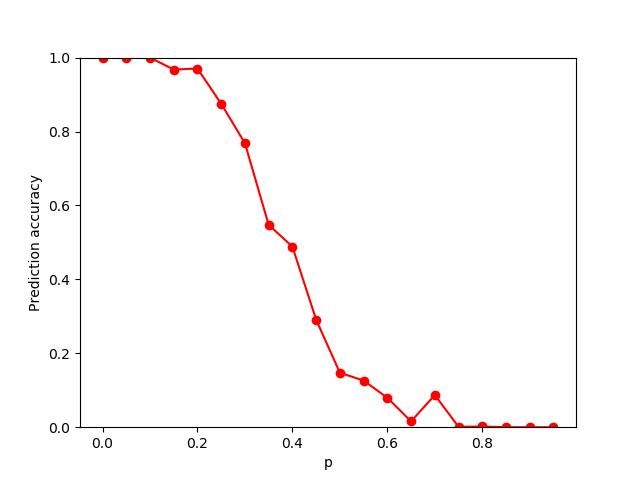
\includegraphics[width=0.75\textwidth]{CompleteGraph_Accuracy_spavg1.png}
\caption{A plot of the data collected using the shortest path metric on the graph constructed from two complete graphs. The graph was constructed using two 200-vertex complete graphs and the probability $q$ of removing edges was set constant at $0.6$.}
\label{fig:complete_graph_plot_shortest_path}
\end{figure}

\begin{figure}[h]
\centering
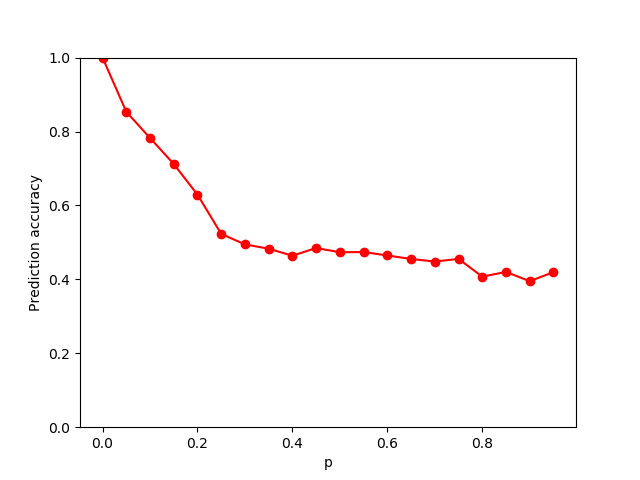
\includegraphics[width=0.75\textwidth]{CompleteGraph_Accuracy_dsdavg1.png}
\caption{A plot of the data collected using the DSD metric on the graph constructed from two complete graphs. The graph was constructed using two 200-vertex complete graphs and the probability $q$ of removing edges was set constant at $0.6$.}
\label{fig:complete_graph_plot_dsd}
\end{figure}

\subsection{Analysis}
\noindent
We do not expect the DSD to do significantly better than the shortest path distance for $p$ from $0$ to $0.5$, as shown in Figure \ref{fig:complete_graph_plot_dsd} and Figure \ref{fig:complete_graph_plot_shortest_path}. This happens because with low probability $p$ of adding edges between components, it is likely that most neighbors of vertices will be within the same component. For example, with probability $p = 0.1$,  there will be significantly fewer edges between the two components compared to edges within each component. This will cause the shortest path metric to predict correctly with a high accuracy since most neighbors of vertices a short distance away will be vertices in the same component. The DSD metric will also predict well since most neighbors of neighbors of a vertex will also be within the same component.

For probability $p$ greater than $0.5$, we expect the DSD metric to outperform the shortest path metric. This is intuitive since with probability of adding edges between components greater than $0.5$, we expect vertices from one component to have more neighbors from the other component than neighbors from the same component. This means that for the shortest path metric, most neighbors a short distance away will have the opposite label. For the DSD metric, however, neighbors of neighbors become equally likely to belong to either component, so the prediction accuracy stays around $50\%$. This clearly shows that the DSD metric considers different aspects of graph structure that the shortest path metric fails to consider.




\section{Distance Histograms}
Small world networks are characterized by their very small characteristic path
length. With this in mind, one would see a very narrow range of values for
pairwise shortest path distances in a small world graph. DSD, however, is more
robust in that its range of possible values degrades more slowly as
characteristic path length increases.

In order to illustate this, we examined Watts-Strogatz graphs with various
values of $p$, starting from the regular ring lattice, $p = 0$. Histograms were
built by computing all of the pairwise distances in the graph using both
shortest path and DSD metrics. Notably, DSD experiences the same degradation as
shortest path distance for graphs with large p, ($p = 0.50$), which corresponds
to Watts-Strogatz graphs with low clustering coefficients, but is relatively
robust for $p = 0.10$, which is where clustering coefficients remain high. This
supports the intuition that DSD is an appropriate distance metric for graphs
that exhibit clustering and hub node behavior.

[These graphs are preliminary and I plan to replace them with density plots and
also to add scale-free networks in addition to performing a comparison on
summary statistics. -- JP]

\begin{figure}[!ht]
\centering
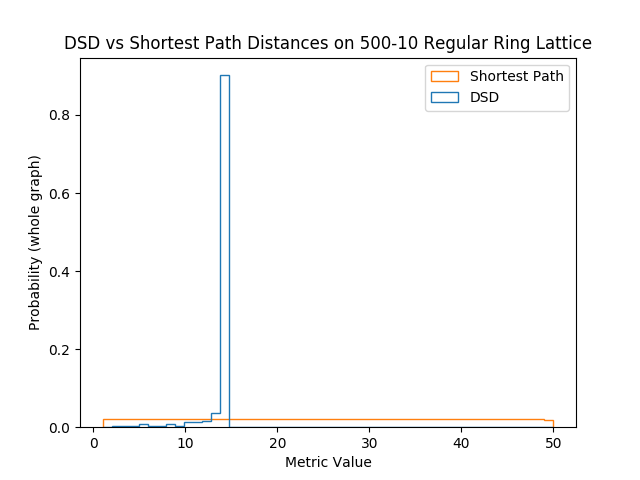
\includegraphics[width=0.85\textwidth]{hist_rrl.png}
\caption{}
\label{fig:hist_rrl}
\end{figure}

\begin{figure}[!ht]
\centering
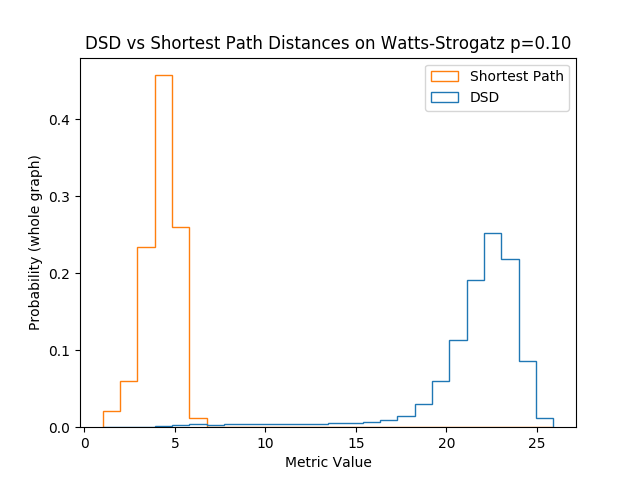
\includegraphics[width=0.85\textwidth]{hist_ws10.png}
\caption{}
\label{fig:hist_ws10}
\end{figure}

\begin{figure}[!ht]
\centering
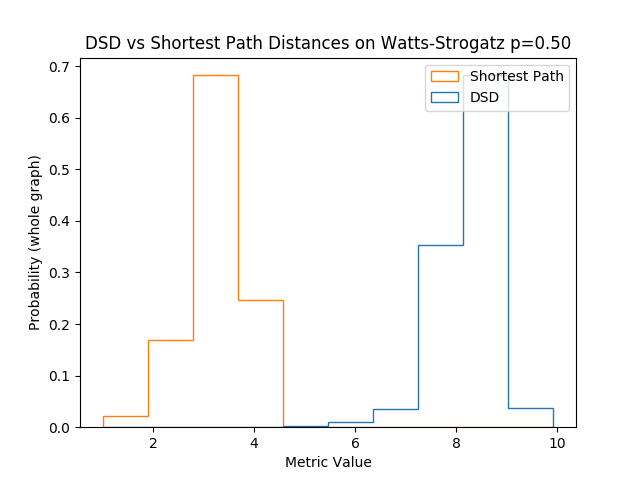
\includegraphics[width=0.85\textwidth]{hist_ws50.png}
\caption{}
\label{fig:hist_ws50}
\end{figure}



\chapter{Analysis of Real-World Data}
% introduce methods used

\section{Selected datasets}

\section{Analysis}


\chapter{Conclusions}

\bibliography{biblio}
\bibliographystyle{plain}

\end{document}
